\scanpage{435}

\unsure{linked} in a much more natural way to the very structure
of the group $\mathcal{M}_{\rho,\sigma}$ and to its homomorphisms
$\xrightarrow{\Theta}G$ and $\chi=\det\circ\Theta$ into $G_m$, namely the
\unsure{integral} subgroup $SR_{\rho,\sigma}$, allowing us to write
even $\mathcal{M}_{\rho,\sigma}^{+}$ as a
\uline{direct product}
\[
\tag{99}
\begin{array}{rccccc}
\mathcal{M}_{\rho,\sigma}^{+}&\simeq&SR_{\rho,\sigma}&\times&
 \unsure{\mathcal{G}|\mathcal{C}}_{\rho,\sigma}^{+}\\
&&\rotatebox{90}{$\simeq$}&&\rotatebox{90}{$\unsure{=|\simeq}$}\\
&&S'T_\rho\times SN'_\sigma&&SG
\end{array}
.
\]
inducing an analogous decomposition
\[
\tag{100}
\left\{
\begin{aligned}
\mathcal{M}_{\rho,\sigma}^{+\circ}
 &\simeq \underset{ST_\rho\times ST_\sigma}{\underbrace{
 SR_{\rho,\sigma}^{\deleted{\unsure{+}}\inserted{\circ}}}}
 \times
 \underset{SG}{\underbrace{\deleted{\unsure{S}}\unsure{\mathcal{G}|\mathcal{C}}_{\rho,\sigma}^{+}}}\\
 &\simeq ST_\rho\times ST_\sigma\times SG,
\end{aligned}
\right.
\]
\margin{this is (46), which I had forgotten along the way\ldots}
who can do better!. On the other hand, the fact that
$R_{\rho,\sigma}\longrightarrow\mathcal{T}_{\rho,\sigma}$ is an
\uline{isogeny} mod $\mu_2$ shows that we have, up to this isogeny, a
``section'' \unsure{of|even}
\deleted{of $\unsure{\mathcal{T}_\rho}$}
\inserted{$\mathcal{M}_{\rho,\sigma}$ itself}
as an extension of $\mathcal{T}_{\rho,\sigma}$ by
$\unsure{\mathcal{G}|\mathcal{C}}_{\rho,\sigma}^{+}\simeq SG$.
In fact, we have
\[
\tag{101}
\left\{
\begin{array}{l}
R_{\rho,\sigma}\cap SG=\mu_2\\[4pt]
\deleted{\text{\unsure{but} }R_{\rho,\sigma}\text{ \unsure{no longer commutes},}}\\[-2pt]
\deleted{\text{\unsure{so we have an exact sequence}}}\\[4pt]
R_{\rho,\sigma}\text{ commutes with }SG
\end{array}
\right.
\]
\hfill (trivial by definition of $R_{\rho,\sigma}$ as
$\operatorname{Ker}\widetilde{\Theta}$

so we have an exact sequence

\mspage{434}

\begin{center}
{\small
434\\
\texttt{https://grothendieck.umontpellier.fr}\\
Université de Montpellier, UMR CNRS 5149, Case courrier 051, Place Eugène Bataillon\\
34095 Montpellier cedex 5 - France
}
\end{center}

\scanpage{436}
\mspage{520}

\begin{samepage}
\noindent(102)
\diagram{\begin{tikzcd}[ampersand replacement=\&,column sep=large,row sep=small]
1\arrow[r]\&\mu_2\arrow[r]\&R_{\rho,\sigma}\times SG\arrow[r]\&
 \mathcal{M}_{\rho,\sigma}\arrow[r]\&1\\
\&\varepsilon\arrow[r,mapsto]\&
 \left(\varepsilon,
 \underset{\inserted{\substack{\Vert\\\varepsilon^{-1}}}}
 {\varepsilon^{\deleted{\unsure{+}}}}\right)
\end{tikzcd}}
\end{samepage}

and likewise

\begin{samepage}
\noindent(103)
\diagram{\begin{tikzcd}[ampersand replacement=\&,column sep=large]
1\arrow[r]\&\mu_2\arrow[r]\&R_{\rho,\sigma}^{\circ}\times SG\arrow[r]\&
\mathcal{M}_{\rho,\sigma}^{\circ}\arrow[r]\&1
\end{tikzcd}}
\end{samepage}

already considered (a little timidly) in (78).
It is decidedly time to make fully explicit the description of
$R_{\rho,\sigma}$ in terms of $T_\rho,N'_\sigma\ldots$ --- we obtain it,
in the context of page~510, \deleted{as} as
\[
\tag{104}
\begin{aligned}
R_{\rho,\sigma}
={}&\left\{
 \left(
 \underset{\substack{\rotatebox{90}{$\in$}\\\Gamma T_0}}{\underline u},
 \underset{\substack{\rotatebox{90}{$\in$}\\\Gamma T_\rho}}{\underline a},
 \underset{\substack{\rotatebox{90}{$\in$}\\\Gamma N'_\sigma}}{\underline b}
 \right)\cdot
 \underset{\substack{\rotatebox{90}{$\in$}\\SG}}{f}
 \ \middle|\ 
 \begin{gathered}
 \det\underline u=\det\underline b=\varepsilon'\det\underline a,
 \quad\varepsilon'{}^2=1\\
 \underline u f=\lambda\qquad(\varepsilon',\lambda\in\Gamma G_m)\\
 (\text{hence }\lambda^2=\det\underline u)
 \end{gathered}\right\}\\[8pt]
\simeq{}&\left\{
 \left(\underset{T_0}{\underline u},
       \underset{T_\rho}{\underline a},
       \underset{N'_\sigma}{\underline b}\deleted{\unsure{)}},
       \underset{G_m}{\lambda}\right)
 \ \middle|\ \det\underline u=\det\underline b
 =\varepsilon'\det\underline a=\lambda^2\right\}\\[8pt]
\simeq{}&\left\{
 \left(\underset{T_\rho}{\underline a},
       \underset{N'_\sigma}{\underline b},
       \underset{G_m}{\lambda}\deleted{\unsure{)}},
       \inserted{\underset{\mu_2}{\varepsilon'}}\right)
 \ \middle|\
 \begin{gathered}
 \inserted{\det\underline b=\varepsilon'\det\underline a=\lambda^2}\\
 \deleted{\unsure{\det\underline b/\det\underline a\in\Gamma\mu_2}}
 \end{gathered}\right\}\\[8pt]
\simeq{}&\left\{
 \left(\underset{T_\rho}{\underline a},
       \underset{N'_\sigma}{\underline b},
       \underset{G_m}{\lambda}\right)
 \ \middle|\ \det\underline b=\lambda^2,\quad
 \det\underline a^2=\det\underline b^2\right\}\\[8pt]
\simeq{}&\left(\deleted{\unsure{\{}}(T_\rho,\delta_\rho^2)
 \times_{G_m}(N'_\sigma,\delta_\sigma^2)\right)_{(\delta_\sigma)}
 \times_{G_m}G_m{}_{(\delta^2)}
\end{aligned}
\]
or more simply, \deleted{which gives}
\inserted{in terms of $\mathcal{T}_{\rho,\sigma}$:}
\[
\deleted{(105)\qquad
\begin{aligned}
 R_{\rho,\sigma}^{\circ}
 &\simeq\left\{
 \left(\underset{T_\rho}{\underline a},
       \underset{T_\sigma}{\underline b},
       \underset{G_m}{\lambda}\right)
 \ \middle|\ \det\underline a=\det\underline b=\lambda^2
 \right\}\\
 &\simeq\unsure{\mathcal{G}|\mathcal{C}}_{\rho,\sigma}^{\circ}
\end{aligned}}
\]

\begin{samepage}
\noindent(105)
\diagram{\begin{tikzcd}[ampersand replacement=\&,column sep=large,row sep=large]
R_{\rho,\sigma}\arrow[r]\arrow[d,"{\kappa}"']\&
 \mathcal{T}_{\rho,\sigma}\arrow[d,"{\chi}"]\&\text{diagram}\\
G_m\arrow[r,"{\delta^2}"']\&G_m\&\text{cartesian}\\[-1em]
\lambda\arrow[r,mapsto]\&\lambda^2
\end{tikzcd}}
\end{samepage},

\mspage{435}

\begin{center}
{\small
435\\
\texttt{https://grothendieck.umontpellier.fr}\\
Université de Montpellier, UMR CNRS 5149, Case courrier 051, Place Eugène Bataillon\\
34095 Montpellier cedex 5 - France
}
\end{center}

\scanpage{437}

fitting into a diagram of exact sequences

\begin{samepage}
\noindent(106)
\diagram{\begin{tikzcd}[ampersand replacement=\&,column sep=large,row sep=large,nodes in empty cells]
\&\&1\arrow[d]\&1\arrow[d]\&\\
\deleted{\unsure{1}}\arrow[r,draw=none,"{\deleted{\longrightarrow}}" description]\&
\deleted{\unsure{\mu_2}}\arrow[r,draw=none,"{\deleted{\longrightarrow}}" description]\&
SR_{\rho,\sigma}\arrow[r,"{\simeq}"]\arrow[d]\arrow[dr,phantom,"{*}" description]\&
\mathcal{T}_{\rho,\sigma}^{+}\arrow[d]
 \arrow[r,draw=none,"{\deleted{\longrightarrow}}" description]\&\deleted{1}\\
1\arrow[r]\&\mu_2\arrow[r]\arrow[d,equal]\&
R_{\rho,\sigma}\arrow[r,"{\mathrm{can.}}"]\arrow[d,"{\kappa}"]\&
\mathcal{T}_{\rho,\sigma}\arrow[r]\arrow[d,"{\chi}"]\&1\\
1\arrow[r]\&\mu_2\arrow[r]\&G_m\arrow[r,"{\lambda\mapsto\lambda^2}"]\arrow[d]\&
G_m\arrow[r]\arrow[d]\&1\\
\&\&1\&1\&
\end{tikzcd}}
\end{samepage}

which is nothing but an explicit description of the upper face
\inserted{$(*)$} of the cubical diagrams (96) ---
\deleted{\unsure{so}} \unsure{we} shall take \unsure{note} that this one
\inserted{is \uline{not} cartesian} --- nor the lower face.
Thus, we construct
\deleted{$\unsure{\mathcal{T}_{\rho,\sigma}}$ and
$\unsure{\mathcal{T}_{\rho,\sigma}|R_{\rho,\sigma}}$}

\noindent(107) group $\mathcal{T}_{\rho,\sigma}$, and \inserted{the homomorphisms}
\diagram{\begin{tikzcd}[ampersand replacement=\&,column sep=large]
\mathcal{T}_{\rho,\sigma}\arrow[r,"{\chi}"]\&G_m
\end{tikzcd}},
\diagram{\begin{tikzcd}[ampersand replacement=\&,column sep=large]
\mathcal{T}_{\rho,\sigma}\arrow[r,"{{(\varepsilon_3,\varepsilon_2)}}"]\&\mu_2\times\mu_2
\end{tikzcd}}

[and thereby thanks to (105).--(106)) $R_{\rho,\sigma}$,
$SR_{\rho,\sigma}\simeq\mathcal{T}_{\rho,\sigma}^{+}$, and also
(by \deleted{\unsure{simplifying}}\inserted{replacing}
$\mathcal{T}_{\rho,\sigma}$ by
$\mathcal{T}_{\rho,\sigma}^{\circ}=\operatorname{Ker}
(\mathcal{T}_{\rho,\sigma}\longrightarrow\mu_2\times\mu_2)$)
$R_{\rho,\sigma}^{\circ}$,
$SR_{\rho,\sigma}^{\circ}\simeq\mathcal{T}_{\rho,\sigma}^{+\circ}$
\unsure{$\Rightarrow$}]
in terms of the groups

\begin{samepage}
\noindent(108) $T_\rho,N'_\sigma$ and of
\diagram{\begin{tikzcd}[ampersand replacement=\&,column sep=large]
T_\rho\arrow[r,"{\delta_\rho}"]\&G_m
\end{tikzcd}},
\diagram{\begin{tikzcd}[ampersand replacement=\&,column sep=large,row sep=large]
N'_\sigma\arrow[r,"{\delta_\sigma}"]\&G_m\\
N'_\sigma\arrow[r,"{\varepsilon_\sigma}"]\&\mu_2
\end{tikzcd}},
\end{samepage}

\mspage{436}

\begin{center}
{\small
436\\
\texttt{https://grothendieck.umontpellier.fr}\\
Université de Montpellier, UMR CNRS 5149, Case courrier 051, Place Eugène Bataillon\\
34095 Montpellier cedex 5 - France
}
\end{center}

\scanpage{438}
\mspage{521}

as a subgroup

\begin{samepage}
\noindent(109)
\diagram{\begin{tikzcd}[ampersand replacement=\&,column sep=small,row sep=large]
\mathcal{T}_{\rho,\sigma}\arrow[r,hook]\&
T_0\arrow[d,"{\delta_0}","{\simeq}"']\&{}\times T_\rho\times N'_\sigma\\
\&G_m\&
\end{tikzcd}}
\end{samepage}
\[
\begin{aligned}
&\phantom{\{}\,\Vert\\[-2pt]
&\left\{\left(\underset{T_0}{\underline u},
              \underset{T_\rho}{\underline a},
              \underset{N'_\sigma}{\underline b}\right)
 \ \middle|\ 
 \delta_0(\underline u)=\delta_\sigma(\underline b)
 =\varepsilon'\delta_\rho(\underline a),\quad\varepsilon'{}^2=1
 \right\}\\
&\hspace{3em}\simeq
 \left\{\left(\underset{T_\rho}{\underline a},
              \underset{N'_\sigma}{\underline b}\right)
 \ \middle|\
 \delta_\rho(\underline a)=\varepsilon'\delta_\sigma(\underline b),
 \quad\varepsilon'{}^2=1\right\}
\end{aligned}
\]
with
\[
\tag{110}
\left\{
\begin{aligned}
\chi(\deleted{\underline u,}\underline a,\underline b)
 &=\unsure{\delta_\sigma|\delta_0}(\underline b)\\
\varepsilon_3(\deleted{\underline u,}\underline a,\underline b)
 &=\delta_\rho(\underline a)/\delta_\sigma(\underline b)\\
\varepsilon_2(\deleted{\underline u,}\underline a,\underline b)
 &=\varepsilon_\sigma(\underline b)
\end{aligned}
\right.
.
\]

With the help of this, we can construct $\mathcal{M}_{\rho,\sigma}$
by (102), and of course the homomorphism

\noindent(111) $\Theta:$\quad
\diagram{\begin{tikzcd}[ampersand replacement=\&,column sep=large]
\mathcal{M}_{\rho,\sigma}\arrow[r]\&G
\end{tikzcd}}

is deduced by passage to the quotient from the obvious homomorphisms

\begin{samepage}
\noindent(112)
\diagram{\begin{tikzcd}[ampersand replacement=\&,column sep=large]
SG\arrow[r,hook]\&G
\end{tikzcd}}
\end{samepage},\qquad
\diagram{\begin{tikzcd}[ampersand replacement=\&,column sep=large,row sep=large]
R_{\rho,\sigma}\arrow[rr]\arrow[dr,"{\kappa}"']\&\&G\\
\&G_m\arrow[r,"{\simeq}"']\&
\uline{\operatorname{Centr}}(G)\arrow[u,hook]
\end{tikzcd}}

\deleted{We have not had to}
whence we deduce the composites

\begin{samepage}
\noindent(113)
\diagram{$\left\{\vcenter{\hbox{\begin{tikzcd}[ampersand replacement=\&,column sep=large,row sep=huge]
\mathcal{M}_{\rho,\sigma}\arrow[r,"{\Theta}"]
 \arrow[rr,bend right=25,"{\widetilde{\Theta}}"']\&
 G\arrow[r]\&PG\\
\mathcal{M}_{\rho,\sigma}\arrow[r,"{\Theta}"]
 \arrow[rr,bend right=25,"{\chi}"']\&
 G\arrow[r,"{\det}"]\&G_m
\end{tikzcd}}}\right.$}
\end{samepage}

We also deduce the exact sequence

\begin{samepage}
\noindent(114)
\diagram{\begin{tikzcd}[ampersand replacement=\&,column sep=large,row sep=large]
1\arrow[r]\&SG\arrow[rr,"{\mathrm{can}}"']\arrow[dr,dashed,"{\mathrm{can}}"']\&\&
\mathcal{M}_{\rho,\sigma}\arrow[r]\&
\mathcal{T}_{\rho,\sigma}\arrow[r]
 \arrow[d,phantom,"{{\rotatebox{90}{$\simeq$}}}" description]\&1\\
\&\&R_{\rho,\sigma}\times SG\arrow[ur,dashed,"{\mathrm{can}}"]\&\&
R_{\rho,\sigma}/\mu_2\&
\end{tikzcd}}
\end{samepage}

\mspage{437}

\begin{center}
{\small
437\\
\texttt{https://grothendieck.umontpellier.fr}\\
Université de Montpellier, UMR CNRS 5149, Case courrier 051, Place Eugène Bataillon\\
34095 Montpellier cedex 5 - France
}
\end{center}

\scanpage{439}

from the description (102), whence composites

\begin{samepage}
\noindent (115)
\diagram{\begin{tikzcd}[ampersand replacement=\&,column sep=large,row sep=small]
 \& \& T_\rho \\
\mathcal{M}_{\rho,\sigma}\arrow[r]
 \& \mathcal{T}_{\rho,\sigma}
   \arrow[ur,"{\mathrm{pr}_1}"]
   \arrow[dr,"{\mathrm{pr}_2}"]
   \arrow[ddr]
 \& \& \\
 \& \& N'_\sigma\arrow[r,"{\det}"] \& G_m \\
 \& \& \mu_2\times\mu_2
\end{tikzcd}}
\end{samepage}

In all this, we have not needed the datum \unsure{of|of the} sections $\rho,\sigma$
of $G$, nor to know anything at all about the way in which $T_\rho,N'_\sigma$
\deleted{are}\inserted{have been} obtained from such sections.
But more delicate \unsure{additional} structures of the
$\mathcal{M}_{\rho,\sigma}$ --- such as the datum of the
\unsure{integral} subgroups $\mathcal{M}_{\rho,\sigma}\unsure{(w)|(\omega)}$ ---
depend on them, and will perhaps allow us to recover them.

\uline{\unsure{Remark|Remark}} The cube (96) is the ``composite'' of two cubical
diagrams, which I am going to make explicit, the first of which completes (95) --- which can
be regarded as a partial diagram of this one:

\mspage{438}

\begin{center}
{\small
438\\
\texttt{https://grothendieck.umontpellier.fr}\\
Université de Montpellier, UMR CNRS 5149, Case courrier 051, Place Eugène Bataillon\\
34095 Montpellier cedex 5 - France
}
\end{center}

\scanpage{440}
\mspage{522}

\begin{samepage}
\noindent (116)
\diagram{\begin{tikzcd}[ampersand replacement=\&,column sep=small,row sep=small]
 \& \& G_m\arrow[ddrr,dashed,"{\lambda\mapsto\lambda^2}"] \& \& \\
 \& R_{\rho,\sigma}
       \arrow[ur,dashed,"{\kappa}"]
       \arrow[drr,hook,"{PG}"]
 \& \& \& \\
 SR_{\rho,\sigma}
       \arrow[ur,hook,"{G_m}"]
       \arrow[rrr,dashed,"{G}"]
       \arrow[ddrr,hook,"{SG}"']
 \& \& \& \mathcal{M}_{\rho,\sigma}\arrow[r,dashed,"{\chi}"] \& G_m \\
 \& \& \& \& \\
 \& \& \mathcal{M}_{\rho,\sigma}^{+}
       \arrow[uur,hook,"{G_m}"]
 \& |[xshift=24pt]| G_m\arrow[ddr,dashed,"{\lambda\mapsto\lambda^2}"] \& \\
 \& R_{\rho,\sigma}^{\circ}
       \arrow[uuuu,hook,"{\mu_2\times\mu_2}"{pos=.25}]
       \arrow[urr,dashed,"{\kappa^{\circ}}"'{pos=.25,xshift=-9pt}]
       \arrow[drr,hook,"{PG}"{pos=.25,xshift=-9pt}]
 \& \& \& \\
 SR_{\rho,\sigma}^{\circ}
       \arrow[uuuu,hook,"{\mu_2\times\mu_2}"']
       \arrow[ur,hook,"{G_m}"]
       \arrow[rrr,dashed,"{G}"]
       \arrow[ddrr,hook,"{SG}"']
 \& \& \& \mathcal{M}_{\rho,\sigma}^{\circ}
       \arrow[uuuu,hook,"{\mu_2\times\mu_2}"{pos=.76}]
       \arrow[r,dashed,"{\chi^{\circ}}"]
 \& G_m \\
 \& \& \& \& \\
 \& \& \mathcal{M}_{\rho,\sigma}^{+\circ}
       \arrow[uuuu,hook,
        "{\begin{gathered}\inserted{\mu_2\times\mu_2}\\
        \deleted{\unsure{\mu_2\times\mu_2}}\end{gathered}}"'{pos=.77,xshift=4pt}]
       \arrow[uur,hook,"{G_m}"]
 \& \& \\
 \& \& \rotatebox{90}{$\simeq$} \& \&
\end{tikzcd}}
\end{samepage}

As in (95)(96), the lower face is deduced from the upper one by
\unsure{passing} to the identity components, the four quotient groups are
isomorphic to one another by the canonical arrows, they are isomorphic to
$\mu_2\times\mu_2$ --- \unsure{itm|item} in the cube \inserted{attached}
below (117). The lateral faces of the cube are cartesian and.
cocartesian, but not the upper faces nor the lower face.

\mspage{439}

\begin{center}
{\small
439\\
\texttt{https://grothendieck.umontpellier.fr}\\
Université de Montpellier, UMR CNRS 5149, Case courrier 051, Place Eugène Bataillon\\
34095 Montpellier cedex 5 - France
}
\end{center}

\scanpage{441}
\mspage{523}

\[
\tag{117}
\diagram{\begin{tikzcd}[ampersand replacement=\&,column sep=1.5em,row sep=2.5em]
 \& \& R_{\rho,\sigma}\arrow[drr,hook,"{{PG}}"] \& \& \& \\
 SR_{\rho,\sigma}\arrow[urr,hook,"{{G_m}}"]\arrow[rrrr,dashed,"{{G}}"]\arrow[dr,hook,"{{SG}}"'] \& \& \& \& \mathcal M_{\rho,\sigma}\arrow[dr,hook] \& \\
 \& \begin{gathered}\mathcal M_{\rho,\sigma}^{+}\\[-.3em]\inserted{\unsure{\simeq SR_{\rho,\sigma}\times SG}}\end{gathered}\arrow[urrr,hook,"{{G_m}}"]\arrow[drr,shift left=.6ex] \& \& \& \& \mathcal T_{\rho,\sigma} \\
 \& \& R_{\rho,\sigma}^{\circ}\arrow[uuu,hook,"{{\mu_2\times\mu_2}}",description,pos=.6]\arrow[drr,hook,"{{SG}}"] \& \mathcal T_{\rho,\sigma}^{+}\arrow[urr,hook,"{{G_m}}"]\arrow[ull,shift left=.6ex] \& \& \\
 \begin{gathered}SR_{\rho,\sigma}^{\circ}\\[-.5em]\rotatebox{90}{$\simeq$}\\[-.5em]ST_\rho\times ST_\sigma\end{gathered}\arrow[uuu,hook,"{{\mu_2\times\mu_2}}"']\arrow[urr,hook,"{{G_m}}"]\arrow[rrrr,dashed,"{{G}}"]\arrow[dr,hook,"{{SG}}"'] \& \& \& \& \mathcal M_{\rho,\sigma}^{\circ}\arrow[uuu,hook,"{{\mu_2\times\mu_2}}"{pos=.25},description]\arrow[dr] \& \\
 \& \mathcal M_{\rho,\sigma}^{+\circ}\arrow[uuu,hook,"{{\mu_2\times\mu_2}}"']\arrow[urrr,hook,"{{G_m}}"] \& \& \& \& \mathcal T_{\rho,\sigma}^{\circ}\arrow[uuu,hook,"{{\mu_2\times\mu_2}}"] \\
 \& \& \& \begin{gathered}\mathcal T_{\rho,\sigma}^{+\circ}\\[-.5em]\rotatebox{90}{$\simeq$}\\[-.5em]ST_\rho\times ST_\sigma\end{gathered}\arrow[uuu,hook,"{{\mu_2\times\mu_2}}"{pos=.28}]\arrow[ull]\arrow[urr,hook,"{{G_m}}"'] \& \&
\end{tikzcd}}
\]

The composite front left face of the cube is of a particularly simple nature, since the middle terms $\mathcal M_{\rho,\sigma}^{+}$, $\mathcal M_{\rho,\sigma}^{+\circ}$ are identified \unsure{simply} with the direct products of the outer terms
\[
\begin{gathered}
SR_{\rho,\sigma}\xrightarrow{\sim}\mathcal T_{\rho,\sigma}^{+}
\quad\text{and}\quad
SR_{\rho,\sigma}^{\circ}\xrightarrow{\sim}\mathcal T_{\rho,\sigma}^{+\circ}\\
\hphantom{SR_{\rho,\sigma}\xrightarrow{\sim}}\simeq S'T_\rho\times SN'_\sigma
\qquad\qquad\simeq ST_\rho\times ST_\sigma
\end{gathered}
\]
with the group $SG$. This is almost the case too for the parallel face (back right face), \inserted{up to the group $\mu_2$ -- this becomes true \unsure{on}} on condition of replacing the \deleted{groups $\mathcal M_{\rho,\sigma}$} middle terms $\mathcal M_{\rho,\sigma}$, $\mathcal M_{\rho,\sigma}^{\circ}$ by the $\mu_2$-coverings
\[
\tag{118}
\mathcal M_{\rho,\sigma}^{\sim}\simeq\unsure{R}_{\rho,\sigma}\times SG,
\qquad \mathcal M_{\rho,\sigma}^{\circ\sim}\simeq R_{\rho,\sigma}^{\circ}\times SG
\]
(cf. \unsure{(107)|(102)}, (103)), which \unsure{will have} also the virtue

\mspage{440}

\begin{center}
{\small
440\\
\texttt{https://grothendieck.umontpellier.fr}\\
Université de Montpellier, UMR CNRS 5149, Case courrier 051, Place Eugène Bataillon\\
34095 Montpellier cedex 5 - France
}
\end{center}

\scanpage{442}

\unsure{delectable} of making the four squares of the upper and lower faces of the two attached cubes cartesian and cocartesian, which they were not before, \unsure{regrettably}.

To finish these scales on the \unsure{radicals} I am going to introduce a canonical homomorphism
\[
\tag{118}
\diagram{\begin{tikzcd}[ampersand replacement=\&]
G_m\arrow[r,hook,"{{i_R}}"] \& R_{\rho,\sigma}^{\circ}
\end{tikzcd}}
\]
via a canonical homomorphism
\[
\tag{119}
\diagram{\begin{tikzcd}[ampersand replacement=\&,row sep=1em]
G_m\arrow[r,hook,"{{i_{\mathcal T}}}"] \& \mathcal T_{\rho,\sigma}^{\circ}\simeq T_\rho\times_{G_m}T_\sigma \\
\lambda\arrow[r,mapsto] \& (\lambda,\lambda)
\end{tikzcd}}
\]
of which \unsure{the composite|the composite} with
\[
\diagram{\begin{tikzcd}[ampersand replacement=\&]
\chi:\mathcal T_{\rho,\sigma}^{\circ}\arrow[r] \& G_m
\end{tikzcd}}
\]
is indeed given by $\lambda\mapsto\lambda^2$ \inserted{(104)}, so that thanks to the description (105) of $R_{\rho,\sigma}$ \inserted{in terms of $\mathcal T_{\rho,\sigma}$} as a fiber product (\unsure{paraphrased} as an expression of $R_{\rho,\sigma}^{\circ}$ in terms of $\mathcal T_{\rho,\sigma}^{\circ}$) we have a unique homomorphism (118), making the diagram commutative

\mspage{441}

\begin{center}
{\small
441\\
\texttt{https://grothendieck.umontpellier.fr}\\
Université de Montpellier, UMR CNRS 5149, Case courrier 051, Place Eugène Bataillon\\
34095 Montpellier cedex 5 - France
}
\end{center}

\scanpage{443}
\mspage{524}

\[
\tag{120}
\diagram{\begin{tikzcd}[ampersand replacement=\&,column sep=3em,row sep=2em]
G_m\arrow[r,"{{i_{\mathcal T}}}"]\arrow[dr,"{{i_R}}"'] \& \mathcal T_{\rho,\sigma}^{\circ} \\
\& R_{\rho,\sigma}^{\circ}\arrow[u,"{{\mathrm{can}}}"']
\end{tikzcd}}
\]
or, more prettily, the diagram of exact sequences
\[
\tag{121}
\diagram{\begin{tikzcd}[ampersand replacement=\&,column sep=1.8em,row sep=2em]
1\arrow[r] \& \mu_2\arrow[r] \& G_m\arrow[r,"{{\lambda\mapsto\lambda^2}}"{yshift=3pt}]\arrow[d,no head] \& G_m\arrow[r,no head] \& 1 \\
\& \& {} \& \&
\end{tikzcd}}.
\]

By construction, we find at once
\[
\tag{122}
\diagram{\begin{tikzcd}[ampersand replacement=\&,column sep=3em]
G_m\arrow[r,"{{i_R}}"]\arrow[rr,bend right=28,"{{\mathrm{id}}}"'] \& R_{\rho,\sigma}^{\circ}\arrow[r,"{{\kappa}}"] \& G_m
\end{tikzcd}}
\]
whence direct product decompositions
\[
\tag{123}
\left\{\begin{aligned}
R_{\rho,\sigma}&\simeq SR_{\rho,\sigma}\times G_m\simeq S'T_\rho\times SN'_\sigma\times G_m\\
R_{\rho,\sigma}^{\circ}&\simeq SR_{\rho,\sigma}^{\circ}\times G_m\\
&\simeq ST_\rho\times ST_\sigma\times G_m
\end{aligned}\right.,
\]
which considerably sharpens (96) with which I was nevertheless so pleased!

In terms of this decomposition, we are going to make explicit the \deleted{\unsure{h}}homomorphism
\[
\diagram{\begin{tikzcd}[ampersand replacement=\&,column sep=1.7em]
\mu_2\arrow[r,hook] \& R_{\rho,\sigma}^{\circ}\subset R_{\rho,\sigma}
\end{tikzcd}}
\quad
\left(\text{\unsure{and }}
\diagram{\begin{tikzcd}[ampersand replacement=\&,column sep=1.4em]
R_{\rho,\sigma}\arrow[r,no head] \& \mathcal T_{\rho,\sigma}
\end{tikzcd}},\ 
\diagram{\begin{tikzcd}[ampersand replacement=\&,column sep=1.4em]
R_{\rho,\sigma}^{\circ}\arrow[r] \& \mathcal T_{\rho,\sigma}^{\circ}
\end{tikzcd}}\right)
\]
which occurs in (102), (103), $\mu_2=R_{\rho,\sigma}\cap SG=R_{\rho,\sigma}^{\circ}\cap SG$,

\deleted{\unsure{We find} in the explicit description (104), that $\mu_2$ corresponds to the $\varepsilon\in\Gamma\mu_2$, \unsure{that} $\varepsilon$ \illegible{2}}

\mspage{442}

\begin{center}
{\small
442\\
\texttt{https://grothendieck.umontpellier.fr}\\
Université de Montpellier, UMR CNRS 5149, Case courrier 051, Place Eugène Bataillon\\
34095 Montpellier cedex 5 - France
}
\end{center}

\scanpage{444}

For the homomorphism
\[
\diagram{\begin{tikzcd}[ampersand replacement=\&,column sep=2em]
R_{\rho,\sigma}\arrow[r] \&
\begin{gathered}
\inserted{\{(\underline a,\underline b)\mid(\det\underline a/\det\underline b)^2=1\}}\\[-.5em]
\rotatebox{90}{$=$}\\[-.5em]
T_{\rho,\sigma}
\end{gathered}\arrow[r,hook] \& T_\rho\times N'_\sigma
\end{tikzcd}}
\]
it suffices to \deleted{define} \inserted{make explicit} the composites
\[
\tag{124}
\left\{\begin{gathered}
\diagram{\begin{tikzcd}[ampersand replacement=\&,column sep=2.2em,row sep=1em]
\& \& T_\rho \\
R_{\rho,\sigma}\arrow[r]\arrow[d,phantom,"{{\rotatebox{90}{$\simeq$}}}" description] \& \unsure{T_{\sigma\sigma}|T_{\rho,\sigma}}\arrow[ur]\arrow[dr] \& \\
S'T_\rho\times SN'_\sigma\times G_m \& \& N'_\sigma
\end{tikzcd}}\\[1em]
\diagram{\begin{tikzcd}[ampersand replacement=\&]
(\underline a,\underline b,\lambda)\arrow[r] \& (\lambda\underline a,\lambda\underline b)
\end{tikzcd}}
\end{gathered}\right.
\]
\margin{we have as well
\[
\underbrace{\det(\lambda\underline a)^2}_{\substack{\lambda^2\\\text{since }(\det\underline a)^2=1}}
=
\underbrace{\det(\lambda\underline b)^2}_{\substack{\lambda^2\ \text{since}\\\det\underline b=1}}
\]}

The kernel of this homomorphism therefore consists of the $(\unsure{\lambda}^{-1},\lambda^{-1},\lambda)$, \unsure{with|where} $\lambda\in\Gamma G_m$ such that $\lambda^{-1}\in\Gamma S'T_\rho$, $\lambda^{-1}\in\Gamma SN'_\sigma$, \deleted{\unsure{that is|and}} i.e. $(\lambda^2)^2=1$ and $\lambda^2=1$, i.e. $\lambda\in\Gamma\mu_2$. Thus
\[
\tag{125}
\left\{\begin{gathered}
\diagram{\begin{tikzcd}[ampersand replacement=\&,column sep=2em]
\begin{gathered}\mu_2\\[-.5em]\rotatebox{90}{$=$}\\[-.5em]R_{\rho,\sigma}\cap SG\end{gathered}\arrow[r,"{{\mathrm{can}}}"] \&
\underbrace{R_{\rho,\sigma}^{\circ}}_{ST_\rho\times ST_\sigma\times G_m}\subset
\underbrace{R_{\rho,\sigma}}_{S'T_\rho\times SN'_\sigma\times G_m}
\end{tikzcd}}\\[1em]
\diagram{\begin{tikzcd}[ampersand replacement=\&]
\lambda\arrow[r,mapsto] \& (\lambda,\lambda,\lambda)
\end{tikzcd}}
\end{gathered}\right.\,.
\]

We thus find the particularly simple explicit description
\[
\tag{126}
\diagram{\begin{tikzcd}[ampersand replacement=\&,column sep=0em,row sep=.8em]
\mathcal T_{\rho,\sigma}\simeq(S'T_\rho\times SN'_\sigma\times G_m)/ \& \mu_2 \\
\& \begin{gathered}\mu_2\ \text{sent ``diagonally'' into the}\\\text{triple product}\end{gathered}\arrow[u]
\end{tikzcd}}
\]

We will note that we have canonical homomorphisms
\[
\diagram{\begin{tikzcd}[ampersand replacement=\&,column sep=1.2em]
\mu_2\arrow[r] \& ST_\rho\subset S'T_\rho
\end{tikzcd}},\quad
\diagram{\begin{tikzcd}[ampersand replacement=\&,column sep=1.2em]
\mu_2\arrow[r] \& ST_\sigma\subset SN'_\sigma
\end{tikzcd}},\quad
\diagram{\begin{tikzcd}[ampersand replacement=\&,column sep=1.2em]
\mu_2\arrow[r,no head] \& G_m
\end{tikzcd}}
\]
(which are used in (125)) whence
\[
\tag{127}
\left\{\begin{gathered}
\diagram{\begin{tikzcd}[ampersand replacement=\&,column sep=1.5em]
\mu_2\times\mu_2\times\mu_2\arrow[r] \&
\underbrace{ST_\rho\times ST_\sigma\times G_m}_{R_{\rho,\sigma}^{\circ}}\subset
\underbrace{S'T_\rho\times SN'_\sigma\times G_m}_{R_{\rho,\sigma}}
\end{tikzcd}}\\
\diagram{\begin{tikzcd}[ampersand replacement=\&]
(\lambda',\lambda'',\lambda)\arrow[r,mapsto] \& (\lambda',\lambda'',\lambda)
\end{tikzcd}}
\end{gathered}\right.
\]
which is none other than (48))

\mspage{443}

\begin{center}
{\small
443\\
\texttt{https://grothendieck.umontpellier.fr}\\
Université de Montpellier, UMR CNRS 5149, Case courrier 051, Place Eugène Bataillon\\
34095 Montpellier cedex 5 - France
}
\end{center}

\scanpage{445}
\mspage{525}

\uline{The Center of} $\mathcal M_{\rho,\sigma}$. It maps under $\widetilde\Theta$ into the center of $PG$ which is trivial, hence
\[
\uline{\mathrm{Cent}}(\mathcal M_{\rho,\sigma})\subset\operatorname{Ker}\widetilde\Theta
=R_{\rho,\sigma}\simeq S'T_\rho\times SN'_\sigma\times G_m
\]
\unsure{whence} obviously. Since $R_{\rho,\sigma}$ commutes with $SG$, and $R_{\rho,\sigma}\,\deleted{\unsure{\times}}\cdot SG=\mathcal M_{\rho,\sigma}$, we conclude
\[
\tag{128}
\uline{\mathrm{Cent}}(\mathcal M_{\rho,\sigma})
=\uline{\mathrm{Cent}}(R_{\rho,\sigma})
=S'T_\rho\times\underset{?}{\uline{\mathrm{Cent}}}(SN'_\sigma)\times G_m
\]
let us therefore determine $\mathrm{Cent}(SN'_\sigma)$. Let us note that
\[
\left\{\begin{array}{l}
\mu_2\simeq N'_\sigma/T_\sigma\quad\text{operates faithfully on }T_\sigma\\
\text{and }T_\sigma=G_m.ST_\sigma
\end{array}\right.
\qquad
\begin{array}{|l}
\text{hence }\underset{\substack{\rotatebox{90}{$\simeq$}\\SN'_\sigma/\unsure{T_\sigma}}}{\mu_2}\text{ operates faithfully}\\
\text{on }ST_\sigma
\end{array}
\]
whence
\[
\tag{129}
\uline{\mathrm{Cent}}(SN'_\sigma)\subset ST_\sigma
\quad\text{whence}\quad
\uline{\mathrm{Cent}}(SN'_\sigma)\simeq(ST_\sigma)^{\mu_2}.
\]

Now we find that
\inserted{\[
\tag{130}
T_\sigma^{\mu_2}\simeq G_m
\]}
\deleted{\unsure{the section} $-1$ of $\mu_2$ operates on $ST_\sigma$ by $x\longrightarrow x^{-1}$, which shows that
\[
\uline{\mathrm{Cent}}(SN'_\sigma)\subset {}_2(ST_\sigma)
=\left\{\unsure{c}\sigma+d\ \middle|\ \begin{array}{l}
-\nu c^2+d^2=1\\
\nu c^2+d^2+2\sigma cd=0
\end{array}\right\}
\]
We have for a section of ${}_2ST_\sigma$, \deleted{\unsure{g|that}}
\[
\begin{array}{ll}
g=c\sigma+d & \det g=-\nu c^2+d^2=1\\
&g^2=\nu c^2+d^2+2cd\sigma=1
\end{array}
\]
\[
\text{i.e.}\quad
\left\{\begin{array}{ll}
-\nu c^2+d^2=1 & \nu c^2+d^2=1\\
2cd=0 &
\end{array}\right.
\]
\deleted{whence} i.e.
\[
\left\{\begin{array}{ll}
2\nu c^2=0 & \text{hence }2c^2=0\quad(\text{since }\nu\text{ invertible}).\\
2cd=0 &\\
-\nu c^2+d^2=1 &
\end{array}\right.
\]
if $2$ invertible this amounts to
\[
\left\{\begin{array}{lll}
&c^2=0&\\
\deleted{\unsure{c^2=0}}&d^2=1&(\text{hence }d\text{ invertible})\\
\deleted{\unsure{d^2=1}}&\unsure{c}d=0&\text{hence }c=0
\end{array}\right.
\]
\unsure{hence}
\[
\boxed{c=0,\ d^2=1}\quad\text{i.e. }g\in\mu_2
\]
\unsure{for|hence if} $2$ invertible.}
\inserted{whence}
\[
\tag{\unsure{131|129}}
\uline{\mathrm{Cent}}(SN'_\sigma)
=\unsure{ST_\sigma}^{\mu_2}
=ST_\sigma\cap G_m
\inserted{=\mu_2}\quad
\deleted{\text{if }2\text{ invertible on }S.}
\]

\deleted{In the general case we will only have
\[
\tag{130}
\mu_2\subset\uline{\mathrm{Cent}}(SN'_\sigma)
\]
and this inclusion induces an isomorphism on the groups of sections in the case where $2$ is a \unsure{regular} section of}

\mspage{444}

\begin{center}
{\small
444\\
\texttt{https://grothendieck.umontpellier.fr}\\
Université de Montpellier, UMR CNRS 5149, Case courrier 051, Place Eugène Bataillon\\
34095 Montpellier cedex 5 - France
}
\end{center}

\scanpage{446}

\deleted{$\uline{\mathcal O}_S$. Let us denote by \deleted{$\unsure{\mu'_2}$}
\[
\tag{131}
\begin{gathered}
\mu'_2\subset ST_\sigma\\[-.5em]
\rotatebox{90}{$=$}\\[-.5em]
\deleted{\unsure{\uline{\mathrm{Cent}}}}(ST_\sigma)^{\mu_2}
\end{gathered}
\]
\unsure{this|a} subgroup of}

whence \unsure{finally|finally}, \unsure{namely|i.e.}:
\[
\tag{128}
\underset{\unsure{=}}{\uline{\mathrm{Cent}}(\mathcal M_{\rho,\sigma})}
\simeq S'T_\rho\times\mu_2\times G_m
\subset R_{\rho,\sigma}\simeq S'T_\rho\times SN'_\sigma\times G_m
\]
whence
\[
\tag{129}
\uline{\mathrm{Cent}}(\mathcal M_{\rho,\sigma})\cap\mathcal M_{\rho,\sigma}^{\circ}
=ST_\rho\times\mu_2\times G_m
\subset R_{\rho,\sigma}^{\circ}\simeq ST_\rho\times ST_\sigma\times G_m
\]

Let us return to the integral sections in the absolute modular case
\[
\tag{130}
R_{\rho,\sigma}(\mathbb Z)\simeq
\underbrace{S'T_\rho(\mathbb Z)}_{\unsure{T_\rho}(\mathbb Z)\simeq\mathbb Z/6\mathbb Z}
\times
\underbrace{SN'_\sigma(\mathbb Z)}_{T_\sigma(\mathbb Z)=\mathbb Z/4\mathbb Z}
\times
\underbrace{G_m(\mathbb Z)}_{\mu_2(\mathbb Z)\simeq\pm1}
\]
\[
\tag{131}
\begin{aligned}
\uline{\mathrm{Cent}}(\mathcal M_{\rho,\sigma})\unsure{[\mathbb Z]|(\mathbb Z)}
&\simeq S'(T_\rho\unsure{[\mathbb Z]|(\mathbb Z)})\times\mu_2(\mathbb Z)\times G_m(\mathbb Z)\\
&\simeq\mathbb Z/6\mathbb Z\times\{\pm1\}\times\{\pm1\}
\end{aligned}
\]
and for the record (cf. (75), p. 514)
\[
\tag{132}
\begin{aligned}
\underbrace{\uline{\mathrm{Cent}}(\mathcal M_{\rho,\sigma}^{\circ})}_{\substack{R_{\rho,\sigma}^{\circ}\\\simeq ST_\rho\times ST_\sigma\times G_m}}(\mathbb Z)
&\simeq ST_\rho(\mathbb Z)\times ST_\sigma(\mathbb Z)\times G_m(\mathbb Z)\\
&\simeq\mathbb Z/6\mathbb Z\times\mathbb Z/4\mathbb Z\times\{\pm1\}.
\end{aligned}
\]

In summary, we have the diagram of \inserted{strict} inclusions of group schemes
\[
\tag{133}
\diagram{\begin{tikzcd}[ampersand replacement=\&,column sep=1.5em,row sep=5em,column sep=9pt,row sep=14pt,execute at begin picture={\fontsize{10}{12}\selectfont}]
\text{dimension }3 \&
\begin{gathered}
\uline{\mathrm{Cent}}(\mathcal M_{\rho,\sigma}^{\circ})=R_{\rho,\sigma}^{\circ}\\
\simeq ST_\rho\times ST_\sigma\times G_m
\end{gathered}
\arrow[rr,hook,"{{{\substack{\text{(quotient}\\\mu_2\times\mu_2\text{)}}}}}"'{yshift=-3pt}]
\&[18pt] \&
\begin{gathered}
R_{\rho,\sigma}\\
\simeq S'T_\rho\times SN'_\sigma\times G_m
\end{gathered}
\&\text{dimension }3\\
\text{dimension }2\&
\begin{gathered}
\uline{\mathrm{Cent}}(\mathcal M_{\rho,\sigma})\cap\mathcal M_{\rho,\sigma}^{\circ}\\
=ST_\rho\times\mu_2\times G_m
\end{gathered}
\arrow[u,hook]\arrow[rr,hook,"{{{\substack{\text{(quotient}\\\mu_2\text{)}}}}}"'{yshift=-3pt}]
\&\&
\begin{gathered}
\uline{\mathrm{Cent}}(\mathcal M_{\rho,\sigma})\\
\simeq S'T_\rho\times\deleted{\unsure{SN'_\sigma}}\inserted{\unsure{\mu_2}}\times G_m)
\end{gathered}
\arrow[u,hook]
\&\text{dimension }2
\end{tikzcd}}
\]

\mspage{445}

\begin{center}
{\small
445\\
\texttt{https://grothendieck.umontpellier.fr}\\
Université de Montpellier, UMR CNRS 5149, Case courrier 051, Place Eugène Bataillon\\
34095 Montpellier cedex 5 - France
}
\end{center}

\scanpage{447}
\mspage{526}

valid in the general case -- and which, in the absolute modular case, induces \unsure{on} the integral points isomorphisms for the two horizontal arrows, \unsure{corresponding} resp. to the two groups
\[
\underset{\unsure{\text{and}}}{(134)}\quad
\left\{
\begin{aligned}
\uline{\mathrm{Cent}}(\mathcal{M}_{\rho,\sigma}^{\circ})(\mathbb{Z})
 &\simeq \mathbb{Z}/6\mathbb{Z}\times\mathbb{Z}/4\mathbb{Z}\times\{\pm1\}\qquad\text{and}\\
\uline{\mathrm{Cent}}(\mathcal{M}_{\rho,\sigma})(\mathbb{Z})
 &\simeq \mathbb{Z}/6\mathbb{Z}\times\{\pm1\}\times\{\pm1\}
\end{aligned}\right.
\]
which is a subgroup of it of index 2.

Finally, for the record \unsure{let us point out} once again the group
\[
(135)\qquad \deleted{\unsure{\pm1\times}}\qquad
\Sigma=\{\pm1\}\times\{\pm1\}\times\{\pm1\}
\]
contained in $\uline{\mathrm{Cent}}(\mathcal{M}_{\rho,\sigma})(\mathbb{Z})$ (of order 8, of index 3), which plays a special role in the arithmetic application, since we will have a canonical homomorphism
\[
(136)\qquad
\boxed{\diagram{\begin{tikzcd}[ampersand replacement=\&,column sep=large]
\mathcal{M}_{0,3}^{\sim}\arrow[r] \& \mathcal{M}_{\rho,\sigma}(\widehat{\mathbb{Z}})/\Sigma
\end{tikzcd}}}\,.
\]

\mspage{446}

\begin{center}
{\small
446\\
\texttt{https://grothendieck.umontpellier.fr}\\
Université de Montpellier, UMR CNRS 5149, Case courrier 051, Place Eugène Bataillon\\
34095 Montpellier cedex 5 - France
}
\end{center}

\scanpage{448}

\margin{\uline{\unsure{Where we define}}\quad\uline{$\mathcal{M}_{\rho,\sigma}$}}

\textcircled{$7^\circ$}\quad Let us make a \unsure{list|little} \unsure{recapitulation|recapitulatory} of the main group homomorphisms considered in the course of section $6^\circ$, involving the group $\mathcal{M}_{\rho,\sigma}$
\[
(134)\qquad
\diagram{\begin{tikzcd}[ampersand replacement=\&,row sep=small,column sep=large]
 \& SG\arrow[dddr,"{j_G}"] \& \& G\arrow[r]\arrow[dr,"{\delta_G=\det_G}"] \& PG\\
 \& \& \& \& G_m\\
 \& S'T_\rho\arrow[dr,"{j_\rho}"] \& \& T_\rho\arrow[r,"{\delta_\rho=\det_{T_\rho}}"{yshift=3pt}] \& G_m\\
\mu_2\arrow[uuur]\arrow[ur]\arrow[dr]\arrow[dddr]
 \& \& \mathcal{M}_{\rho,\sigma}\arrow[uuur,"{\Theta=\Theta_G}"]\arrow[ur,"{\Theta_\rho}"]\arrow[dr,"{\Theta_\sigma}"]\arrow[dddr,"{\varepsilon_3}"'] \& \& \\
 \& SN'_\sigma\arrow[ur,"{j_\sigma}"'] \& \& N'_\sigma\arrow[r,"{\delta'_\sigma=\det_{T_\sigma}}"{yshift=3pt}]\arrow[dr,"{\varepsilon_\sigma}"] \& G_m\\
 \& \& \& \& \mu_2\\
 \& G_m\arrow[uuur,hook,"{j_\mu}"'] \& \& \mu_2 \&
\end{tikzcd}}
\]

Let us note that this diagram can be reconstructed (with the essential properties which we are going to \unsure{pass} in \unsure{review}) from the data
\[
(135)\quad
\left\{\begin{gathered}
\diagram{\begin{tikzcd}[ampersand replacement=\&,column sep=large]
G_m\arrow[r,"{i_\rho}"] \& T_\rho\arrow[r,"{\delta_\rho}"] \& G_m \& (\delta_\rho i_\rho(\lambda)=\lambda^2)
\end{tikzcd}}\\[1em]
\diagram{\begin{tikzcd}[ampersand replacement=\&,column sep=large]
G_m\arrow[r,"{i_\sigma}"] \& N'_\sigma\arrow[r,"{\delta_\sigma}"] \& G_m \& (\delta_\sigma i_\sigma(\lambda)=\lambda^2)
\end{tikzcd}}\\[1em]
\diagram{\begin{tikzcd}[ampersand replacement=\&,column sep=large]
 \& N'_\sigma\arrow[r,"{\varepsilon_\sigma}"] \& \mu_2 \& \varepsilon_\sigma i_\sigma(\lambda)=1
\end{tikzcd}}\\[1em]
\diagram{\deleted{\begin{tikzcd}[ampersand replacement=\&,column sep=large]
1\arrow[r] \& G_m\arrow[r]\arrow[dr,phantom,"{\text{cartesian}}" description] \& G\arrow[r] \& PG\arrow[r] \& 1\\
1\arrow[r] \& \mu_2\arrow[u,hook]\arrow[r] \& SG\arrow[u,hook]\arrow[r] \& PG\arrow[u,equal]\arrow[r] \& 1
\end{tikzcd}}}
\end{gathered}\right.
\]
in addition to the \unsure{familiar} \unsure{datum}
\[
(136)\qquad
\diagram{\begin{tikzcd}[ampersand replacement=\&,column sep=large,row sep=large]
 \& 1 \& 1 \& \&\\
 \& G_m\arrow[u]\arrow[r,equal] \& G_m\arrow[u] \& \&\\
1\arrow[r] \& G_m\arrow[u,"{\lambda\mapsto\lambda^2}"]\arrow[r,hook,"{\unsure{j}}"] \& G\arrow[u,"{\delta_G}"]\arrow[r] \& PG\arrow[r] \& 1\\
1\arrow[r] \& \mu_2\arrow[u,hook]\arrow[r] \& SG\arrow[u,hook]\arrow[r] \& PG\arrow[u,equal]\arrow[r] \& 1\\
 \& 1\arrow[u] \& \unsure{0|1}\arrow[u] \& \&
\end{tikzcd}}
\]

\mspage{447}

\begin{center}
{\small
447\\
\texttt{https://grothendieck.umontpellier.fr}\\
Université de Montpellier, UMR CNRS 5149, Case courrier 051, Place Eugène Bataillon\\
34095 Montpellier cedex 5 - France
}
\end{center}

\scanpage{449}
\mspage{527}

Let us recall that we define, in terms of (135)
\[
(137)\quad
\left\{\begin{gathered}
ST_\rho=\mathrm{Ker}\,\delta_\rho,\quad S'T_\rho=\mathrm{Ker}\,\delta_\rho^2\\
T_\sigma=\mathrm{Ker}\,\varepsilon_\sigma,\quad
SN'_\sigma=\mathrm{Ker}\,\delta'_\sigma,\quad
ST_\sigma=SN'_\sigma\cap T_\sigma=\mathrm{Ker}\,\delta_\sigma\\
\hfill(\delta_\sigma=\delta'_\sigma|T_\sigma)\\[.5em]
\diagram{\begin{tikzcd}[ampersand replacement=\&,column sep=small]
\mu_2\arrow[r] \& ST_\rho\subset S'T_\rho \& \text{as composite} \& \mu_2\subset G_m\arrow[r,"{i_\rho}"{yshift=3pt}] \& T_\sigma\\
\mu_2\arrow[r] \& ST_\sigma\subset SN'_\sigma \& \rule{2cm}{.3pt} \& \mu_2\subset G_m\arrow[r,"{i_\sigma}"{yshift=3pt}] \& T_\sigma
\end{tikzcd}}
\end{gathered}\right.,
\]
which determines the left-hand part of diagram (134), where $\mathcal{M}_{\rho,\sigma}$ can be considered (and defined) as \inserted{\unsure{quotient of the}} \deleted{amalgamated} sum of the four factors $SG,S'T_\rho,SN'_\sigma,G_m$, \inserted{by $\mu_2$ \unsure{embedding} itself in it diagonally.}

This makes it possible in principle to reduce the description of the four fundamental morphisms from $\mathcal{M}_{\rho,\sigma}$ in (134) -- $\Theta_G,\Theta_\rho,\Theta_\sigma$ and $\varepsilon_{\unsure{3|2}}$ -- to their composites with the four homomorphisms
$j_G,j_\rho,j_\sigma,j_\mu$ -- subject to checking \inserted{that the}\deleted{\unsure{images}} of the four composites \deleted{\unsure{coincide}}\inserted{\unsure{commute}, and that their product of} \deleted{\unsure{that the|on the}}\inserted{their values on the images of an $\deleted{\unsure{\varepsilon|\equiv}}\ \varepsilon\in\Gamma\mu_2$ is trivial.} \deleted{four subgroups $\mu_2$} We will have
\[
(138)\quad
\left\{\begin{gathered}
\diagram{\begin{tikzcd}[ampersand replacement=\&,column sep=large]
\Theta_Gj_G: \& SG\arrow[r,hook] \& G,\quad\text{canonical inclusion}\quad(136)
\end{tikzcd}}\\[.5em]
\diagram{\deleted{\begin{tikzcd}[ampersand replacement=\&,column sep=small]
\unsure{\Theta_Gj_\rho}: \& \unsure{S'T_\rho}\arrow[r,hook] \& \unsure{T_\rho}\arrow[r,"{\delta_\rho}"{yshift=3pt}] \& G_m\arrow[r,hook,"{\unsure{j}}"] \& G
\end{tikzcd}}}\\[.5em]
\Theta_Gj_\rho,\ \Theta_Gj_\sigma\qquad\text{trivial}\\[.5em]
\diagram{\begin{tikzcd}[ampersand replacement=\&,column sep=large]
\Theta_Gj_\mu: \& G_m\arrow[r] \& G_m\quad\text{canonical inclusion}
\end{tikzcd}}
\end{gathered}\right.
\]
(conditions of \unsure{compatibility|compatibilities} satisfied !)

\mspage{448}

\begin{center}
{\small
448\\
\texttt{https://grothendieck.umontpellier.fr}\\
Université de Montpellier, UMR CNRS 5149, Case courrier 051, Place Eugène Bataillon\\
34095 Montpellier cedex 5 - France
}
\end{center}

\scanpage{450}

\[
(\unsure{139|135})\quad
\left\{\begin{gathered}
\Theta_\rho j_G\ \deleted{\text{trivial}},\quad \Theta_\rho j_\sigma\quad\text{trivial}\\[.5em]
\diagram{\begin{tikzcd}[ampersand replacement=\&,column sep=large]
\Theta_\rho j_\rho:\ \& S'T_\sigma\arrow[r,hook] \& T_\rho\quad\text{inclusion}
\end{tikzcd}}\\[.5em]
\diagram{\begin{tikzcd}[ampersand replacement=\&,column sep=large]
\Theta_\rho j_\mu:\ \& G_m\arrow[r,"{i_\rho}"] \& T_\rho
\end{tikzcd}}
\end{gathered}\right.
\]
trivial compatibilities,
\[
(140)\quad
\left\{\begin{gathered}
\Theta_\sigma j_G,\quad\Theta_\sigma j_\rho\quad\text{trivial}\\[.5em]
\diagram{\begin{tikzcd}[ampersand replacement=\&,column sep=large]
\Theta_\sigma j_\sigma:\ \& SN'_\sigma\arrow[r,hook] \& N'_\sigma\quad\text{inclusion}
\end{tikzcd}}\\[.5em]
\diagram{\begin{tikzcd}[ampersand replacement=\&,column sep=large]
\Theta_\sigma j_\mu:\ \& G_m\arrow[r,"{i_\sigma}"] \& N'_\sigma
\end{tikzcd}}
\end{gathered}\right.
\]
trivial compatibilities,
\[
(141)\quad
\left\{\begin{gathered}
\deleted{\unsure{\Theta}}\varepsilon_3 j_G,\quad
\deleted{\varepsilon_3j_\rho}\inserted{\varepsilon_3j_\sigma},\quad
\varepsilon_3j_\mu\quad\text{trivial}\\[.5em]
\diagram{\begin{tikzcd}[ampersand replacement=\&,column sep=large]
\varepsilon_3j_\rho:\ \& S'T_\rho\arrow[r,"{\delta_\rho}"] \& \mu_2
\end{tikzcd}}\\[-.2em]
\deleted{\unsure{\varepsilon_3j_\sigma}}
\end{gathered}\right.\,.
\]

We therefore define, in terms of (134)
\[
(142)\quad
\left\{\begin{gathered}
\diagram{\begin{tikzcd}[ampersand replacement=\&,row sep=large,column sep=large]
\mathcal{M}_{\rho,\sigma}\arrow[rr,"{\varepsilon_2}"]\arrow[dr,"{\Theta_\sigma}"'] \& \& \mu_2 \& \varepsilon_2=\varepsilon_\sigma\circ\Theta_\sigma\,.\\
\& N'_\sigma\arrow[ur,"{\varepsilon_\sigma}"'] \& \&
\end{tikzcd}}\\[1.5em]
\diagram{\begin{tikzcd}[ampersand replacement=\&,row sep=large,column sep=large]
\mathcal{M}_{\rho,\sigma}\arrow[rr,"{\chi}"]\arrow[dr,"{\Theta_G}"'] \& \& G_m \& \chi=\delta_G\circ\Theta_G\\
\& G\arrow[ur,"{\delta_G=\det}"'] \& \&
\end{tikzcd}}\\[1.5em]
\diagram{\begin{tikzcd}[ampersand replacement=\&,row sep=large,column sep=large]
\mathcal{M}_{\rho,\sigma}\arrow[rr,"{\widetilde{\Theta}}"]\arrow[dr,"{\Theta_G}"'] \& \& PG \& \widetilde{\Theta}=\mathrm{can}\circ\Theta_G\\
\& G\arrow[ur,"{\mathrm{can}}"'] \& \&
\end{tikzcd}}
\end{gathered}\right.
\]
we shall therefore have
\[
(143)\qquad
\diagram{\begin{tikzcd}[ampersand replacement=\&,column sep=huge]
\mathcal{M}_{\rho,\sigma}\arrow[r,"{(\chi,\varepsilon_3,\varepsilon_2)}"] \& G_m\times\mu_2\times\mu_2
\end{tikzcd}}\,,
\]
\hfill epimorphism

\mspage{449}

\begin{center}
{\small
449\\
\texttt{https://grothendieck.umontpellier.fr}\\
Université de Montpellier, UMR CNRS 5149, Case courrier 051, Place Eugène Bataillon\\
34095 Montpellier cedex 5 - France
}
\end{center}

\scanpage{451}
\mspage{528}

and the other two composites $\delta_\rho\Theta_\rho$ and $\delta'_\sigma\Theta_\sigma$ of (134) are made explicit \unsure{therefore|then} by the formulas
\[
(144)\quad
\left\{\begin{aligned}
\delta'_\sigma\Theta_\sigma&=\chi\quad\bigl(\overset{\unsure{\mathrm{dfn}}}{=}\delta_G\Theta_G\bigr)\\
\delta_\rho\Theta_\rho(g)&=\varepsilon_3(g)\chi(g)
\end{aligned}\right.
\]
In terms of (143) we define
\[
(145)\quad
\left\{\begin{aligned}
\mathcal{M}_{\rho,\sigma}^{+}
&=\mathrm{Ker}\left(\diagram{\begin{tikzcd}[ampersand replacement=\&,column sep=large]
\mathcal{M}_{\rho,\sigma}\arrow[r,"{\chi}"]\&G_m
\end{tikzcd}}\right)\\[1em]
\mathcal{M}_{\rho,\sigma}^{\circ}
&=\mathrm{Ker}\left(\diagram{\begin{tikzcd}[ampersand replacement=\&,column sep=large]
\mathcal{M}_{\rho,\sigma}\arrow[r,"{(\varepsilon_3,\varepsilon_2)}"]\&\mu_2\times\mu_2
\end{tikzcd}}\right)\\[1em]
\mathcal{M}_{\rho,\sigma}^{+\circ}
&=\mathcal{M}_{\rho,\sigma}^{+}\cap\mathcal{M}_{\rho,\sigma}^{\circ}
=\mathrm{Ker}\left(\diagram{\begin{tikzcd}[ampersand replacement=\&,column sep=large]
\mathcal{M}_{\rho,\sigma}\arrow[r,"{(\chi,\varepsilon_3,\varepsilon_2)}"]\&G_m\times\mu_2\times\mu_2
\end{tikzcd}}\right)
\end{aligned}\right.,
\]

we define
\[
(146)\quad
\left\{\begin{aligned}
R_{\rho,\sigma}
&=\mathrm{Ker}\left(\diagram{\begin{tikzcd}[ampersand replacement=\&,column sep=large]
\mathcal{M}_{\rho,\sigma}\arrow[r,"{\widetilde{\Theta}}"]\&PG
\end{tikzcd}}\right)\\[1em]
R_{\rho,\sigma}^{\circ}
&=\mathcal{M}_{\rho,\sigma}\cap R_{\rho,\sigma}
=\mathrm{Ker}\left(\diagram{\begin{tikzcd}[ampersand replacement=\&,column sep=large]
\mathcal{M}_{\rho,\sigma}^{\circ}\arrow[r,"{\widetilde{\Theta}^{\circ}}"]\&PG
\end{tikzcd}}\right)\\[1em]
SR_{\rho,\sigma}
&=\mathrm{Ker}\left(\diagram{\begin{tikzcd}[ampersand replacement=\&,column sep=large]
\mathcal{M}_{\rho,\sigma}\arrow[r,"{\Theta}"]\&G
\end{tikzcd}}\right)\\[1em]
SR_{\rho,\sigma}^{\circ+}
&=\mathrm{Ker}\left(\diagram{\begin{tikzcd}[ampersand replacement=\&,column sep=large]
\mathcal{M}_{\rho,\sigma}\arrow[r,"{(\Theta,\varepsilon_3,\varepsilon_2)}"]\&G\times\mu_2\times\mu_2
\end{tikzcd}}\right)\\[.5em]
&=SR_{\rho,\sigma}\cap R_{\rho,\sigma}^{\circ}
\end{aligned}\right.
\]

whence the cartesian and cocartesian squares (94), and more richly, the \inserted{\uline{\unsure{prismatic} --}} cubical diagrams (\unsure{95|05}) (96) (116) (117), and the dévissages
\[
(147)\quad
\left\{\begin{aligned}
R_{\rho,\sigma}&\simeq S'T_\rho\times SN'_\sigma\times G_m\\[.5em]
R_{\rho,\sigma}^{\circ}&\simeq ST_\rho\times ST_\sigma\times G_m\\[.5em]
SR_{\rho,\sigma}&\simeq S'T_\rho\times SN'_\sigma\times1\\[.5em]
SR_{\rho,\sigma}^{\circ}&\simeq ST_\rho\times ST_\sigma\times1
\end{aligned}\right.,
\]
\margin{whose meaning is evident from diagram (134)}

\mspage{450}

\begin{center}
{\small
450\\
\texttt{https://grothendieck.umontpellier.fr}\\
Université de Montpellier, UMR CNRS 5149, Case courrier 051, Place Eugène Bataillon\\
34095 Montpellier cedex 5 - France
}
\end{center}

\scanpage{452}

\[
\tag{148}
\left\{
\diagram{\begin{tikzcd}[ampersand replacement=\&,column sep=large,row sep=large]
1 \arrow[r,dash] \& \mu_2 \arrow[r] \arrow[d,equal] \& R_{\rho,\sigma}\times SG \arrow[r,dash] \& \mathcal{M}_{\rho,\sigma} \arrow[r,dash] \& 1 \\
1 \arrow[r,dash] \& \mu_2 \arrow[r,dash] \& R_{\rho,\sigma}^{\circ}\times SG \arrow[r,dash] \arrow[u,hook,no head,"{{\unsure{\mu_2\times\mu_2}}}"'] \& \mathcal{M}_{\rho,\sigma}^{\circ} \arrow[r,dash] \arrow[u,hook,no head,"{{\unsure{\mu_2\times\mu_2}}}"'] \& 1
\end{tikzcd}}
\right.\ ,
\]
\margin{this is here the \uline{\unsure{definition}} of $\mathcal{M}_{\rho,\sigma}$}

\[
\tag{149}
\left\{\begin{aligned}
\mathcal{M}_{\rho,\sigma}^{+}&\simeq SR_{\rho,\sigma}\times SG\\
\mathcal{M}_{\rho,\sigma}^{+\circ}&\simeq SR_{\rho,\sigma}^{\circ}\times SG
\end{aligned}\right.\ ,
\]

Finally, \unsure{let us define}
\[
\tag*{(150).}
\left\{\begin{aligned}
\mathcal{T}_{\rho,\sigma}&\simeq
\mathcal{M}_{\rho,\sigma}/
\underset{\substack{\Vert\,\mathrm{d\acute ef}\\\unsure{\mathcal{G}|\mathcal{C}}_{\rho,\sigma}^{+}}}{\uline{SG}},\\
\mathcal{T}_{\rho,\sigma}^{\circ}&=
\mathcal{M}_{\rho,\sigma}^{\circ}/SG
=\operatorname{Ker}(\mathcal{T}_{\rho,\sigma}\longrightarrow\mu_2\times\mu_2)\\
\mathcal{T}_{\rho,\sigma}^{+}&=
\mathcal{M}_{\rho,\sigma}^{+}/SG
=\operatorname{Ker}(\mathcal{T}_{\rho,\sigma}\longrightarrow G_m)\\
\mathcal{T}_{\rho,\sigma}^{+\circ}&=
\mathcal{M}_{\rho,\sigma}^{+\circ}/SG
=\operatorname{Ker}(\mathcal{T}_{\rho,\sigma}\longrightarrow\uline{G_m}\times\mu_2\times\mu_2)\\
&=\mathcal{T}_{\rho,\sigma}^{\circ}\cap\mathcal{T}_{\rho,\sigma}^{+}
\quad\text{in }\mathcal{T}_{\rho,\sigma},
\end{aligned}\right.
\]
whence extension structures
\diagram{\begin{tikzcd}[ampersand replacement=\&]
1\arrow[r] \& SG\arrow[r,dash] \& \mathcal{M}_{\rho,\sigma}\arrow[r,dash] \& \mathcal{T}_{\rho,\sigma}\arrow[r,dash] \& 1
\end{tikzcd}}
etc (\unsure{itm|item} with
$\begin{array}{l}
\mathcal{M}_{\rho,\sigma}^{\circ},\mathcal{T}_{\rho,\sigma}^{\circ}\\
\mathcal{M}_{\rho,\sigma}^{+},\mathcal{T}_{\rho,\sigma}^{+}\\
\mathcal{M}_{\rho,\sigma}^{+\circ},\mathcal{T}_{\rho,\sigma}^{+\circ}
\end{array}$)

and exact sequences
\diagram{\begin{tikzcd}[ampersand replacement=\&]
1\arrow[r,dash] \& \mathcal{T}_{\rho,\sigma}^{\circ}\arrow[r,dash] \& \mathcal{T}_{\rho,\sigma}\arrow[r] \& \mu_2\times\mu_2\arrow[r,dash] \& 1
\end{tikzcd}}
etc (\unsure{itm|item} for
$\begin{array}{l}
\mathcal{T}_{\rho,\sigma}^{+}\subset\mathcal{T}_{\rho,\sigma}\\
\mathcal{T}_{\rho,\sigma}^{+\circ}\subset\mathcal{T}_{\rho,\sigma}\\
\mathcal{T}_{\rho,\sigma}^{+\circ}\subset\mathcal{T}_{\rho,\sigma}^{+}\\
\mathcal{T}_{\rho,\sigma}^{+\circ}\subset\mathcal{T}_{\rho,\sigma}^{\circ}
\end{array}$

\mspage{451}

\begin{center}
{\small
451\\
\texttt{https://grothendieck.umontpellier.fr}\\
Université de Montpellier, UMR CNRS 5149, Case courrier 051, Place Eugène Bataillon\\
34095 Montpellier cedex 5 - France
}
\end{center}

\scanpage{453}
\mspage{529}

finally \unsure{isomorphisms}
\[
\tag{151}
\left\{\begin{gathered}
\diagram{\begin{tikzcd}[ampersand replacement=\&,column sep=large]
R_{\rho,\sigma}/\mu_2 \arrow[r,"{\sim}"] \& \mathcal{T}_{\rho,\sigma}\\
R_{\rho,\sigma}^{\circ}/\mu_2 \arrow[r,"{\sim}"] \& \mathcal{T}_{\rho,\sigma}^{\circ}\\
SR_{\rho,\sigma} \arrow[r,phantom,"{\simeq}"] \& \mathcal{T}_{\rho,\sigma}^{+}\\
SR_{\rho,\sigma}^{\circ} \arrow[r,phantom,"{\simeq}"] \& \mathcal{T}_{\rho,\sigma}^{+\circ}
\end{tikzcd}}
\end{gathered}\right.\,.
\]

\figure{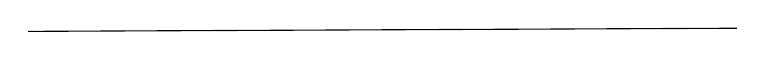
\begin{tikzpicture}\draw (0,0)--(9,0.04);\end{tikzpicture}}

\figure{
\begin{tikzpicture}[baseline=(n.base)]
\node (n) at (0,0) {$8^{\circ}$};
\draw (0,0) ellipse (0.35 and 0.31);
\end{tikzpicture}}
If $U$ is an element of $\mathcal{M}_{\rho,\sigma}$, we
associate to it its images under $\Theta=\Theta_G$, $\Theta_\rho$, $\Theta_\sigma$, and under
\deleted{$\unsure{\varepsilon_3,\varepsilon_2}$}
$\chi$, $\varepsilon_3$, $\varepsilon_2$, we denote them respectively
\[
\tag{152}
\left\{\begin{array}{l}
\uline{U}\in\Gamma G\\[4pt]
\uline{a}\ \unsure{\in}\Gamma T_\rho\\[4pt]
\uline{b}\in\Gamma N'_\sigma\\[4pt]
\figure{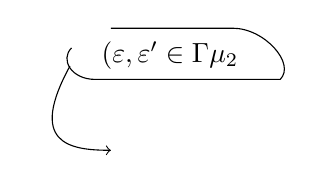
\begin{tikzpicture}[baseline=(e.base)]
\node[inner sep=3pt] (e) at (0,0) {$(\varepsilon,\varepsilon'\in\Gamma\mu_2$};
\draw (-1.25,0.1) .. controls (-1.4,-0.05) and (-1.25,-0.3) .. (-0.95,-0.3)
 -- (1.4,-0.3) .. controls (1.6,-0.1) and (1.2,0.35) .. (0.8,0.35) -- (-0.75,0.35);
\draw[->] (-1.27,-0.13) .. controls (-1.8,-1.1) and (-1.3,-1.2) .. (-0.75,-1.2);
\end{tikzpicture}}\\[4pt]
\mu\in\Gamma G_m
\end{array}\right.
\]

\margin{\unsure{satisfying}
\[
\tag{152'}
\left\{\begin{aligned}
\mu&=\delta_G(\uline{U})=\unsure{\delta'_\sigma|\delta_\sigma}(\uline{b})=\varepsilon'\delta_\rho(a)\\
\unsure{\varepsilon'|\varepsilon}&=\varepsilon_\sigma(\uline{b})
\end{aligned}\right.
\]
thus these quantities are determined by the mere
\unsure{knowledge} of $\uline{U},\uline{a},\uline{b}$}

\margin{\figure{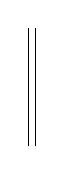
\begin{tikzpicture}
\draw (0,0)--(0,1.5);\draw (0.09,0)--(0.09,1.5);
\end{tikzpicture}}
It would be necessary to make explicit that the \unsure{equalities|relations} (152)' \uline{characterize}
$\mathcal{M}_{\rho,\sigma}$ as a subgroup of $G\times T_\rho\times N'_\sigma$
-- it would be necessary to carry out the verification, to
see \unsure{whether we have not} \unsure{forgotten}, in
\unsure{(135)} some \unsure{hyp$^{\mathrm{ses}}$} to be made\ldots}

\margin{\uline{N.B.} $G^{\pm1}\overset{\mathrm{d\acute ef}}{=}\operatorname{Ker}\delta_G^2$}

with notations from \S\ 46 and following.
\unsure{missing} however, \unsure{in|for} the perspective \unsure{of the} \unsure{integral points},
are the elements previously denoted
\diagram{\begin{tikzcd}[ampersand replacement=\&,column sep=small,row sep=small]
\uline{u} \& \alpha \& \beta \& \alpha_0 \& \beta_0 \& f\arrow[lllll,bend right=28]
\end{tikzcd}}
, with
\[
\left|\begin{aligned}
u&\in\Gamma\unsure{T_0}\subset\Gamma G\\
\alpha,\alpha_0&\in\Gamma G^{\pm1}\subset\Gamma G\\
\beta,\beta_0,f&\in\Gamma SG.
\end{aligned}\right.
\]
linked \inserted{to one another and to the preceding ones,} by relations
\[
\left\{\diagram{\begin{tikzcd}[ampersand replacement=\&,row sep=small,column sep=normal]
\alpha=\uline{u}\,\uline{a}^{-1}
\& {}\arrow[d,dash,start anchor=north,end anchor=south]
\& |[yshift=-0.8em]|{\text{i.e.}\quad\uline{u}=\alpha\unsure{\overline{a}}=\beta b.}\\
\beta=\uline{u}\,\uline{b}^{-1} \& {} \& \\
\uline{U}=f^{-1}\uline{u}
\arrow[uu,bend left=80,start anchor=west,end anchor=west]
\arrow[u,bend left=70,start anchor=west,end anchor=west] \& \& \\
\alpha_0=f^{-1}\alpha \& \& \text{i.e.}\quad\alpha=f\alpha_0\\
\beta_0=f^{-1}\beta \& \& \text{i.e.}\quad\beta=f\beta_0
\end{tikzcd}}\right.
\]
\margin{formulas \uline{in $G$}}

\margin{\uline{N.B.} of these \unsure{6 quantities} (153),
$\uline{u}$ is distinguished by the fact of being
\uline{\unsure{multiplicative}}
(like the quantities (152))}

\margin{We could introduce
\[
\left\{\begin{aligned}
\xi&=\alpha\rho(\alpha)^{-1}\\
\eta&=\unsure{\varepsilon}\,\beta\sigma(\beta)^{-1}
\end{aligned}\right.
\quad\unsure{(153)}
\]
\[
\begin{aligned}
g&=\alpha_0\rho(\alpha_0)^{-1}\\
h&=\unsure{\varepsilon}\,\beta_0\unsure{\sigma}(\beta_0)^{-1}
\end{aligned}
\]
but \unsure{little} do we \unsure{care} here.}

\mspage{452}

\begin{center}
{\small
452\\
\texttt{https://grothendieck.umontpellier.fr}\\
Université de Montpellier, UMR CNRS 5149, Case courrier 051, Place Eugène Bataillon\\
34095 Montpellier cedex 5 - France
}
\end{center}
